\documentclass[a4paper,12pt]{article}

% --- Tiếng Việt + mã UTF-8 ---
\usepackage[utf8]{inputenc}
\usepackage[T5]{fontenc}
\usepackage[vietnamese]{babel}

% --- Bố cục trang ---
\usepackage{geometry}
\geometry{top=2.5cm, bottom=2.5cm, left=3cm, right=2cm}

% --- Toán ---
\usepackage{amsmath}
\usepackage{amssymb}

% --- Hình ảnh (logo bìa + đồ thị) ---
\usepackage{graphicx}
\graphicspath{{img/}}

% --- Khung viền bìa ---
\usepackage{tikz}
\usetikzlibrary{calc}

% --- Bảng ---
\usepackage{array}

% --- Liên kết ---
\usepackage{hyperref}

\begin{document}

% ================= KHUNG VIỀN BÌA =================
\begin{tikzpicture}[remember picture, overlay]
  \draw[line width=1.2pt, color=blue!40!black]
    ($(current page.north west)+(1.1cm,-1.1cm)$)
    rectangle ($(current page.south east)+(-1.1cm,1.1cm)$);
  \draw[line width=0.5pt, color=blue!40!black]
    ($(current page.north west)+(1.35cm,-1.35cm)$)
    rectangle ($(current page.south east)+(-1.35cm,1.35cm)$);
\end{tikzpicture}

% ================= TRANG BÌA =================
\begin{center}

\includegraphics[width=4cm]{SGU-LOGO.png}

TRƯỜNG ĐẠI HỌC SÀI GÒN

KHOA TOÁN -- ỨNG DỤNG

\textbf{BÀI TẬP: HỒI QUY LOGISTIC VÀ ĐỒ THỊ TÍNH TOÁN}

Môn: Học sâu (Deep Learning)

Họ và tên: Đinh Quang Minh

MSSV: 3123580024

Lớp: DDU1231

Ngành: Khoa học dữ liệu

Giảng viên hướng dẫn: TS. Đỗ Như Tài

Học kỳ: Học kỳ I, năm học 2026

TP. Hồ Chí Minh, tháng 10 năm 2026
\end{center}

\newpage

% ================= PHƯƠNG PHÁP =================
\section*{PHƯƠNG PHÁP THỰC HIỆN}

Bài làm được hoàn thành theo quy trình kết hợp giải tay và công cụ AI như sau:

\begin{enumerate}
  \item \textbf{Giải tay toàn bộ trước:} tính toán chi tiết từng câu trên giấy,
        ghi lại đầy đủ các bước trung gian và đáp số cuối cùng.
  \item \textbf{Dùng AI agent tạo \LaTeX{}:} agent đọc đề gốc, dựng tài liệu,
        chuyển bảng biểu và công thức sang \LaTeX{} và hoàn thành đáp án.
  \item \textbf{Đối chiếu với bài giải tay:} so từng đáp số, tính lại các bước
        trung gian đến khi khớp hoàn toàn.
  \item \textbf{Kiểm chứng bằng code:} hai câu yêu cầu lập trình (Bài 2j, Bài 3h)
        được chạy thật bằng PyTorch, kết quả và đồ thị đưa vào bài.
\end{enumerate}

\newpage
\section*{BÀI 1. HỒI QUY LOGISTIC PHÂN LOẠI GIỚI TÍNH TRẺ SƠ SINH}

Một cơ sở y tế thu thập dữ liệu cân nặng và giới tính trẻ sơ sinh, cần xây dựng mô hình
Logistic Regression dự đoán giới tính từ cân nặng khi sinh. Tập huấn luyện:

\begin{center}
\begin{tabular}{|c|c|c|c|}
\hline
STT & Cân nặng $x_i$ (kg) & Giới tính & Nhãn $y_i$ \\
\hline
1 & 2.4 & Nữ & 0 \\
2 & 3.3 & Nam & 1 \\
3 & 3.2 & Nam & 1 \\
4 & 2.5 & Nữ & 0 \\
\hline
\end{tabular}
\end{center}

Mô hình: $\hat{y}_i = h_\theta(x_i) = \sigma(\theta_0 + \theta_1 x_i)$ với
$\sigma(z) = \dfrac{1}{1+e^{-z}}$ (nhãn 0 là nữ, 1 là nam; $\hat{y}_i$ là xác suất trẻ
thuộc lớp nam).

Hàm mất mát Binary Cross-Entropy:
\[ J(\theta_0,\theta_1) = -\frac{1}{m}\sum_{i=1}^{m}\bigl[y_i\ln(\hat{y}_i) + (1-y_i)\ln(1-\hat{y}_i)\bigr],
\qquad m = 4. \]
Khởi tạo $\theta_0^{(0)} = 0.5$, $\theta_1^{(0)} = 0.5$, tốc độ học $\alpha = 0.2$;
quy tắc cập nhật $\theta_j^{(t+1)} = \theta_j^{(t)} - \alpha\dfrac{\partial J}{\partial\theta_j}$.

\subsection*{a) Đầu vào tuyến tính và xác suất dự đoán}

Đầu vào tuyến tính và xác suất dự đoán của mô hình:
\[ z_i = \theta_0 + \theta_1 x_i, \qquad \hat{y}_i = \sigma(z_i) = \frac{1}{1+e^{-z_i}}. \]

Với $\theta_0^{(0)} = \theta_1^{(0)} = 0.5$, ta có $z_i = 0.5 + 0.5x_i$:
\begin{center}
\begin{tabular}{|c|c|c|c|}
\hline
Mẫu & $x_i$ & $z_i$ & $\hat{y}_i = \sigma(z_i)$ \\
\hline
1 & 2.4 & $0.5+0.5\cdot 2.4 = 1.70$ & 0.845535 \\
2 & 3.3 & $0.5+0.5\cdot 3.3 = 2.15$ & 0.895669 \\
3 & 3.2 & $0.5+0.5\cdot 3.2 = 2.10$ & 0.890903 \\
4 & 2.5 & $0.5+0.5\cdot 2.5 = 1.75$ & 0.851953 \\
\hline
\end{tabular}
\end{center}

\subsection*{b) Binary Cross-Entropy Loss từng mẫu và trung bình}

Loss từng mẫu $l_i = -\bigl[y_i\ln(\hat{y}_i) + (1-y_i)\ln(1-\hat{y}_i)\bigr]$:

\begin{center}
\begin{tabular}{|c|c|c|c|}
\hline
Mẫu & $y_i$ & Cách tính $l_i$ & $l_i$ \\
\hline
1 & 0 & $-\ln(1-0.845535) = -\ln(0.154465)$ & 1.867786 \\
2 & 1 & $-\ln(0.895669)$ & 0.110185 \\
3 & 1 & $-\ln(0.890903)$ & 0.115520 \\
4 & 0 & $-\ln(1-0.851953) = -\ln(0.148047)$ & 1.910224 \\
\hline
\end{tabular}
\end{center}

Hàm mất mát trung bình tại thời điểm khởi tạo:
\[ J\bigl(\theta_0^{(0)},\theta_1^{(0)}\bigr) = \frac{1}{4}(1.867786+0.110185+0.115520+1.910224)
= \frac{4.003715}{4} = 1.000929. \]

\subsection*{c) Chứng minh công thức đạo hàm}

Ta chứng minh cho từng mẫu rồi lấy trung bình. Với
$l_i = -\bigl[y_i\ln\hat{y}_i + (1-y_i)\ln(1-\hat{y}_i)\bigr]$ và $\hat{y}_i = \sigma(z_i)$:

\textbf{Bước 1 — đạo hàm theo $\hat{y}_i$:}
\[ \frac{\partial l_i}{\partial \hat{y}_i}
= -\left[\frac{y_i}{\hat{y}_i} - \frac{1-y_i}{1-\hat{y}_i}\right]. \]

\textbf{Bước 2 — đạo hàm sigmoid:} $\sigma'(z) = \sigma(z)\bigl(1-\sigma(z)\bigr)$, nên
\[ \frac{\partial \hat{y}_i}{\partial z_i} = \hat{y}_i(1-\hat{y}_i). \]

\textbf{Bước 3 — quy tắc dây chuyền theo $z_i$:}
\[ \frac{\partial l_i}{\partial z_i}
= \frac{\partial l_i}{\partial \hat{y}_i}\cdot\frac{\partial \hat{y}_i}{\partial z_i}
= -\left[\frac{y_i}{\hat{y}_i} - \frac{1-y_i}{1-\hat{y}_i}\right]\hat{y}_i(1-\hat{y}_i). \]
Rút gọn:
\[ = -\bigl[y_i(1-\hat{y}_i) - (1-y_i)\hat{y}_i\bigr]
= -\bigl[y_i - y_i\hat{y}_i - \hat{y}_i + y_i\hat{y}_i\bigr]
= -\bigl[y_i - \hat{y}_i\bigr] = \hat{y}_i - y_i. \]

\textbf{Bước 4 — theo tham số:} vì $\dfrac{\partial z_i}{\partial\theta_0} = 1$ và
$\dfrac{\partial z_i}{\partial\theta_1} = x_i$:
\[ \frac{\partial J}{\partial\theta_0}
= \frac{1}{m}\sum_{i=1}^{m}\frac{\partial l_i}{\partial z_i}\cdot 1
= \frac{1}{m}\sum_{i=1}^{m}(\hat{y}_i - y_i), \]
\[ \frac{\partial J}{\partial\theta_1}
= \frac{1}{m}\sum_{i=1}^{m}\frac{\partial l_i}{\partial z_i}\cdot x_i
= \frac{1}{m}\sum_{i=1}^{m}(\hat{y}_i - y_i)\,x_i. \qquad \blacksquare \]

\subsection*{d) Gradient tại khởi tạo và lần cập nhật thứ nhất}

Bảng $\hat{y}_i - y_i$ và $(\hat{y}_i - y_i)x_i$:
\begin{center}
\begin{tabular}{|c|c|c|c|}
\hline
Mẫu & $\hat{y}_i$ & $\hat{y}_i - y_i$ & $(\hat{y}_i-y_i)x_i$ \\
\hline
1 & 0.845535 & $0.845535$ & $0.845535\cdot 2.4 = 2.029284$ \\
2 & 0.895669 & $-0.104331$ & $-0.104331\cdot 3.3 = -0.344292$ \\
3 & 0.890903 & $-0.109097$ & $-0.109097\cdot 3.2 = -0.349110$ \\
4 & 0.851953 & $0.851953$ & $0.851953\cdot 2.5 = 2.129883$ \\
\hline
\end{tabular}
\end{center}

\[ \frac{\partial J}{\partial\theta_0}
= \frac{0.845535-0.104331-0.109097+0.851953}{4} = \frac{1.484060}{4} = 0.371015, \]
\[ \frac{\partial J}{\partial\theta_1}
= \frac{2.029284-0.344292-0.349110+2.129883}{4} = \frac{3.465765}{4} = 0.866441. \]

Cập nhật thứ nhất:
\[ \theta_0^{(1)} = 0.5 - 0.2\cdot 0.371015 = 0.425797, \]
\[ \theta_1^{(1)} = 0.5 - 0.2\cdot 0.866441 = 0.326712. \]

\subsection*{e) Lần cập nhật thứ hai}

Với $\theta_0^{(1)} = 0.425797$, $\theta_1^{(1)} = 0.326712$, tính lại
$z_i = 0.425797 + 0.326712\,x_i$:
\begin{center}
\begin{tabular}{|c|c|c|c|c|}
\hline
Mẫu & $x_i$ & $z_i$ & $\hat{y}_i$ & $\hat{y}_i - y_i$ \\
\hline
1 & 2.4 & 1.209906 & 0.770282 & $0.770282$ \\
2 & 3.3 & 1.503947 & 0.818162 & $-0.181838$ \\
3 & 3.2 & 1.471275 & 0.813251 & $-0.186749$ \\
4 & 2.5 & 1.242577 & 0.776012 & $0.776012$ \\
\hline
\end{tabular}
\end{center}

\[ \frac{\partial J}{\partial\theta_0}
= \frac{0.770282-0.181838-0.186749+0.776012}{4} = 0.294427, \]
\[ \frac{\partial J}{\partial\theta_1}
= \frac{0.770282\cdot2.4 -0.181838\cdot3.3 -0.186749\cdot3.2 +0.776012\cdot2.5}{4}
= \frac{2.591045}{4} = 0.647761. \]

Cập nhật thứ hai:
\[ \theta_0^{(2)} = 0.425797 - 0.2\cdot 0.294427 = 0.366912, \]
\[ \theta_1^{(2)} = 0.326712 - 0.2\cdot 0.647762 = 0.197160. \]

\subsection*{f) Hàm mất mát tại ba thời điểm}

\begin{center}
\begin{tabular}{|c|c|}
\hline
Thời điểm & $J$ \\
\hline
Trước cập nhật & 1.000929 \\
Sau lần cập nhật 1 & 0.843619 \\
Sau lần cập nhật 2 & 0.758527 \\
\hline
\end{tabular}
\end{center}

\textbf{Nhận xét:} hàm mất mát giảm đơn điệu qua từng lần cập nhật
($1.000929 \to 0.843619 \to 0.758527$), cho thấy Gradient Descent đang hội tụ đúng hướng;
mức giảm vẫn còn lớn nên cần nhiều vòng lặp hơn để đạt cực tiểu.

\subsection*{g) Dự đoán với mô hình sau hai lần cập nhật}

Mô hình sau hai lần cập nhật: $\hat{y} = \sigma(0.366912 + 0.197160\,x)$.

Với $x = 2.8$: $z = 0.366912 + 0.197160\cdot 2.8 = 0.918960$,
$\hat{y} = \sigma(0.918960) = 0.714830 \geq 0.5 \Rightarrow$ \textbf{Nam}.

Với $x = 3.5$: $z = 0.366912 + 0.197160\cdot 3.5 = 1.056972$,
$\hat{y} = \sigma(1.056972) = 0.742111 \geq 0.5 \Rightarrow$ \textbf{Nam}.

Vậy mô hình dự đoán cả hai trẻ đều là \textbf{nam}.

\subsection*{h) Đồ thị tính toán (Computation Graph)}

Đồ thị cho một mẫu huấn luyện, gồm các nút $z_i$, $\hat{y}_i$ và $L_i$ (BCE).
Mũi tên liền (xanh) là chiều lan truyền tiến; mũi tên nét đứt (đỏ) là chiều lan truyền
ngược kèm đạo hàm cục bộ tại mỗi nút:

\begin{center}
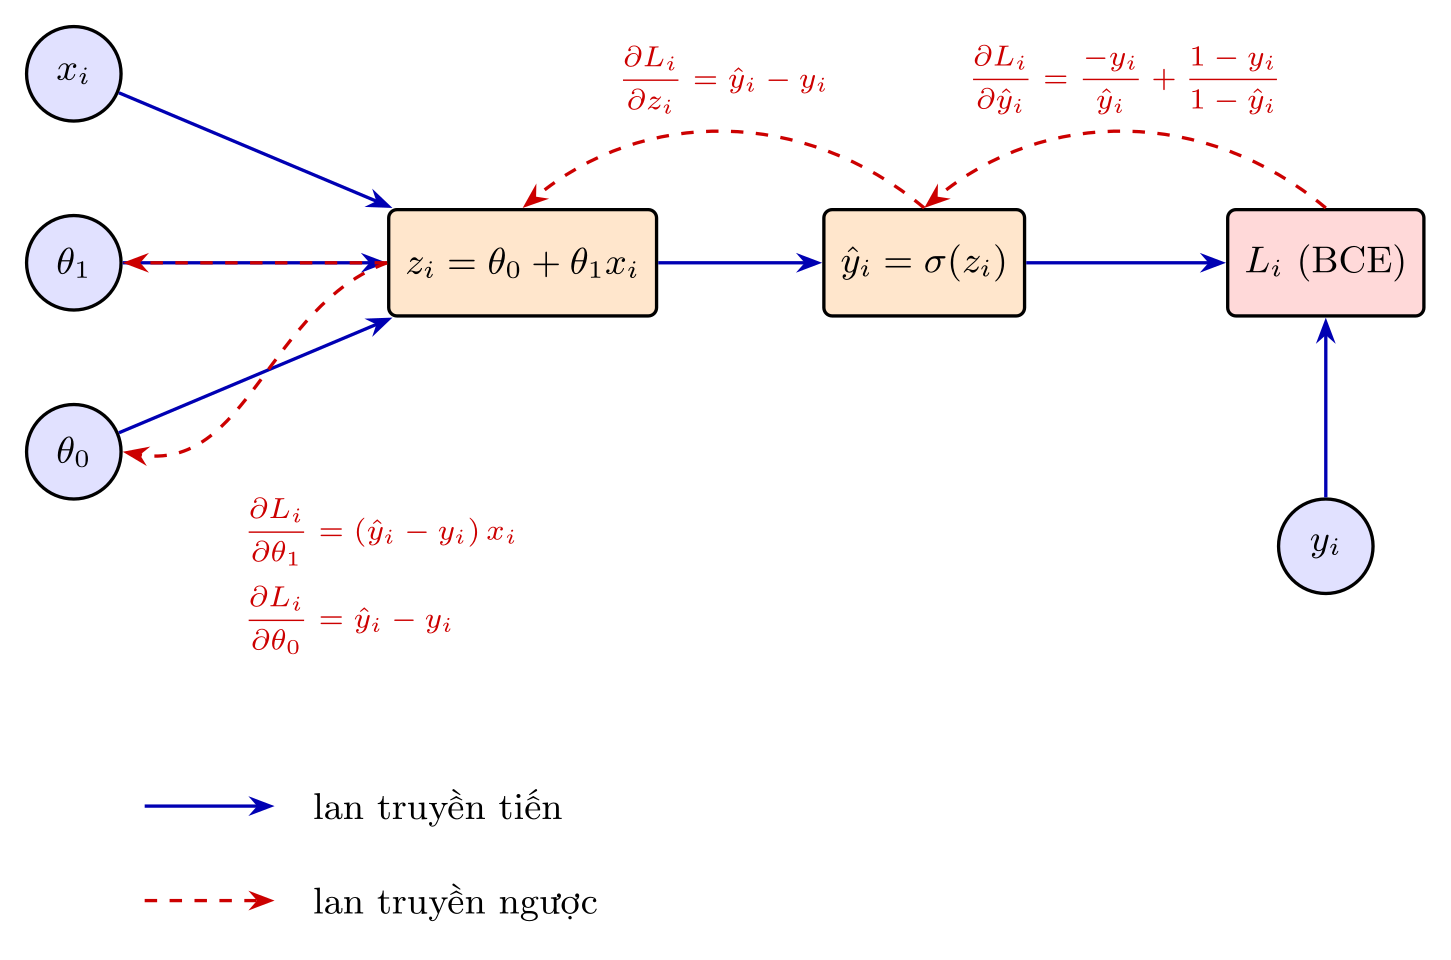
\includegraphics[width=0.98\textwidth]{b1_graph.png}
\end{center}

\newpage
\section*{BÀI 2. HỒI QUY LOGISTIC DỰ ĐOÁN ĐÁNH GIÁ PHIM}

Hệ thống đánh giá phim thu thập thời lượng và mức độ đánh giá của 14 bộ phim
(nhóm Tốt G, nhãn 1; nhóm Không tốt B, nhãn 0). Tập huấn luyện:

\begin{center}
\begin{tabular}{|c|c|c|c||c|c|c|c|}
\hline
STT & $x_i$ (phút) & ĐG & $y_i$ & STT & $x_i$ (phút) & ĐG & $y_i$ \\
\hline
1 & 132 & G & 1 & 8 & 106 & B & 0 \\
2 & 141 & G & 1 & 9 & 102 & B & 0 \\
3 & 88 & B & 0 & 10 & 143 & G & 1 \\
4 & 154 & G & 1 & 11 & 76 & B & 0 \\
5 & 151 & G & 1 & 12 & 168 & G & 1 \\
6 & 102 & B & 0 & 13 & 94 & B & 0 \\
7 & 119 & B & 0 & 14 & 186 & G & 1 \\
\hline
\end{tabular}
\end{center}

Mô hình: $\hat{y}_i = \sigma(w x_i + b)$ với $\sigma(z) = \dfrac{1}{1+e^{-z}}$.
Hàm mất mát BCE: $J(w,b) = -\dfrac{1}{m}\sum_{i=1}^{m}\bigl[y_i\ln\hat{y}_i + (1-y_i)\ln(1-\hat{y}_i)\bigr]$,
$m = 14$. Đặc trưng được chuẩn hóa: $x'_i = \dfrac{x_i - 130}{50}$, mô hình dùng $x'_i$.
Khởi tạo $w^{(0)} = 0$, $b^{(0)} = 0$, $\alpha = 0.2$.

\subsection*{a) Đầu vào, đầu ra, tham số và biểu diễn dữ liệu}

\begin{itemize}
  \item \textbf{Đầu vào:} $x_i$ là thời lượng bộ phim thứ $i$ (phút), dùng dạng chuẩn hóa $x'_i$.
  \item \textbf{Đầu ra:} $y_i \in \{0,1\}$ là nhãn thực tế (1 = phim tốt, 0 = phim không tốt);
        mô hình dự đoán $\hat{y}_i$ là xác suất phim thuộc nhóm tốt.
  \item \textbf{Tham số cần học:} trọng số $w$ và hệ số chặn $b$.
\end{itemize}

Biểu diễn 14 mẫu trên hệ trục (trục hoành là thời lượng, trục tung là nhãn):

\begin{center}
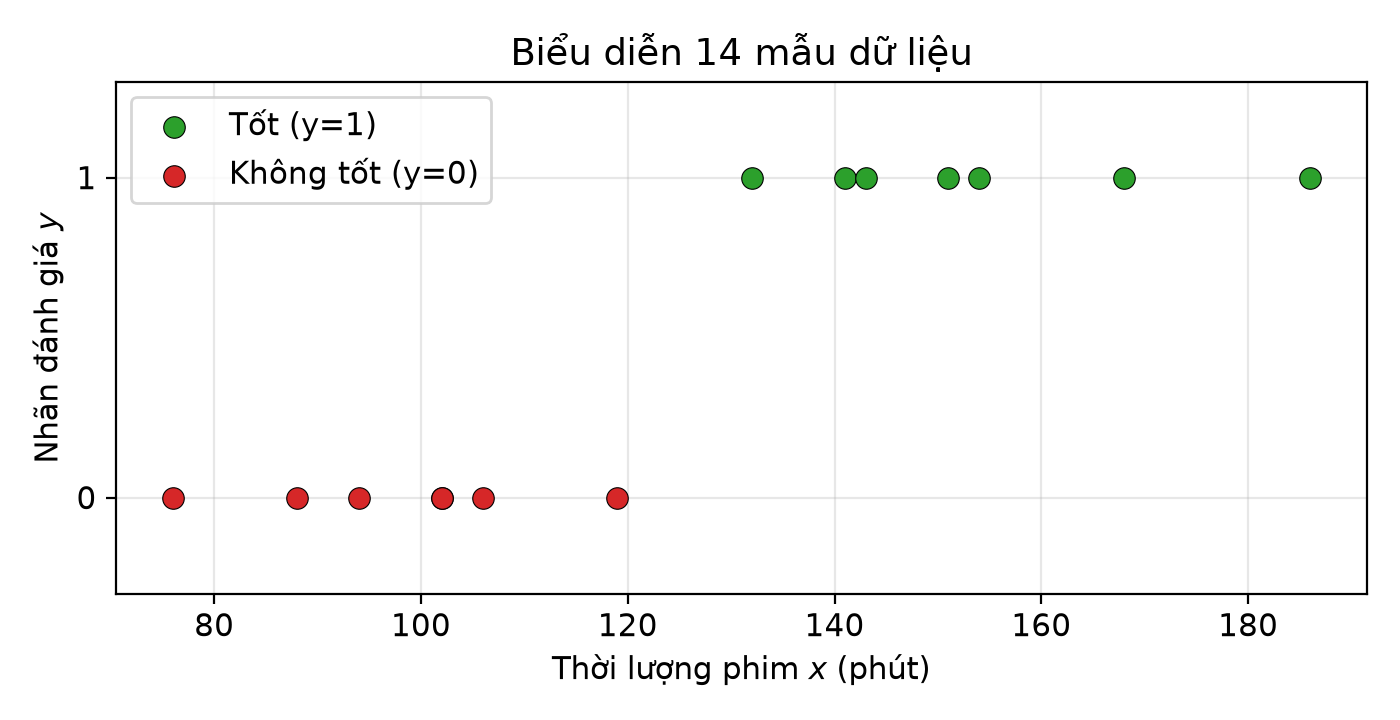
\includegraphics[width=0.82\textwidth]{b2_scatter.png}
\end{center}

\subsection*{b) Đặc trưng chuẩn hóa, $z_i$ và $\hat{y}_i$ tại thời điểm khởi tạo}

Bảng giá trị $x'_i$ và các đại lượng tại $w^{(0)} = b^{(0)} = 0$:

\begin{center}
\begin{tabular}{|c|c|c|c|c|c|}
\hline
STT & $x_i$ & $x'_i = \dfrac{x_i-130}{50}$ & $y_i$ & $z_i = wx'_i+b$ & $\hat{y}_i = \sigma(z_i)$ \\
\hline
1 & 132 & 0.04 & 1 & 0 & 0.5 \\
2 & 141 & 0.22 & 1 & 0 & 0.5 \\
3 & 88 & $-0.84$ & 0 & 0 & 0.5 \\
4 & 154 & 0.48 & 1 & 0 & 0.5 \\
5 & 151 & 0.42 & 1 & 0 & 0.5 \\
6 & 102 & $-0.56$ & 0 & 0 & 0.5 \\
7 & 119 & $-0.22$ & 0 & 0 & 0.5 \\
8 & 106 & $-0.48$ & 0 & 0 & 0.5 \\
9 & 102 & $-0.56$ & 0 & 0 & 0.5 \\
10 & 143 & 0.26 & 1 & 0 & 0.5 \\
11 & 76 & $-1.08$ & 0 & 0 & 0.5 \\
12 & 168 & 0.76 & 1 & 0 & 0.5 \\
13 & 94 & $-0.72$ & 0 & 0 & 0.5 \\
14 & 186 & 1.12 & 1 & 0 & 0.5 \\
\hline
\end{tabular}
\end{center}

Vì $w^{(0)} = b^{(0)} = 0$ nên $z_i = 0$ và $\hat{y}_i = \sigma(0) = 0.5$ cho mọi mẫu.

\subsection*{c) Binary Cross-Entropy Loss từng mẫu và trung bình}

Với $\hat{y}_i = 0.5$ cho mọi mẫu, loss từng mẫu đều bằng:
\[ l_i = -\bigl[y_i\ln 0.5 + (1-y_i)\ln 0.5\bigr] = -\ln 0.5 = \ln 2 \approx 0.693147. \]

Hàm mất mát trung bình:
\[ J(w^{(0)}, b^{(0)}) = \frac{1}{14}\sum_{i=1}^{14} 0.693147 = 0.693147. \]

\subsection*{d) Chứng minh biểu thức gradient}

Lập luận giống Bài 1, với $z_i = wx'_i + b$:
\[ \frac{\partial l_i}{\partial z_i} = \hat{y}_i - y_i, \qquad
   \frac{\partial z_i}{\partial w} = x'_i, \qquad
   \frac{\partial z_i}{\partial b} = 1. \]
Suy ra:
\[ \frac{\partial J}{\partial w}
= \frac{1}{m}\sum_{i=1}^{m}(\hat{y}_i - y_i)\,x'_i, \qquad
   \frac{\partial J}{\partial b}
= \frac{1}{m}\sum_{i=1}^{m}(\hat{y}_i - y_i). \qquad \blacksquare \]

\subsection*{e) Hai lần cập nhật Batch Gradient Descent}

\textbf{Lần 1} (tại $w = b = 0$, $\hat{y}_i - y_i = 0.5 - y_i$):
\[ \frac{\partial J}{\partial w} = \frac{1}{14}\sum(0.5-y_i)x'_i = -0.277143, \qquad
   \frac{\partial J}{\partial b} = \frac{1}{14}\sum(0.5-y_i) = 0 \]
(vì có đúng 7 mẫu $y=1$ và 7 mẫu $y=0$ nên tổng $\sum(0.5-y_i) = 0$).
\[ w^{(1)} = 0 - 0.2\cdot(-0.277143) = 0.055429, \qquad
   b^{(1)} = 0 - 0.2\cdot 0 = 0. \]

\textbf{Lần 2} (tại $w^{(1)} = 0.055429$, $b^{(1)} = 0$):
\[ \frac{\partial J}{\partial w} = -0.271549, \qquad
   \frac{\partial J}{\partial b} = -0.001148. \]
\[ w^{(2)} = 0.055429 - 0.2\cdot(-0.271549) = 0.109738, \qquad
   b^{(2)} = 0 - 0.2\cdot(-0.001148) = 0.000230. \]

Giá trị hàm mất mát sau mỗi lần cập nhật:

\begin{center}
\begin{tabular}{|c|c|}
\hline
Thời điểm & $J$ \\
\hline
Khởi tạo & 0.693147 \\
Sau cập nhật 1 & 0.677941 \\
Sau cập nhật 2 & 0.663341 \\
\hline
\end{tabular}
\end{center}

\subsection*{f) Mô hình sau hai lần cập nhật và dự đoán}

Phương trình mô hình: $\hat{y} = \sigma(0.109738\,x' + 0.000230)$,
tức $\hat{y} = \sigma\!\left(0.109738\cdot\dfrac{x-130}{50} + 0.000230\right)$.

\begin{itemize}
  \item Với $x = 125$: $x' = -0.1$, $z = -0.010744$, $\hat{y} = \sigma(-0.010744) = 0.497314$.
        Vì $\hat{y} < 0.5$ nên dự đoán \textbf{không tốt}.
  \item Với $x = 160$: $x' = 0.6$, $z = 0.066073$, $\hat{y} = \sigma(0.066073) = 0.516512$.
        Vì $\hat{y} \geq 0.5$ nên dự đoán \textbf{tốt}.
\end{itemize}

\subsection*{g) Phân loại 14 phim, ma trận nhầm lẫn và các chỉ số}

Với ngưỡng 0.5, nhãn dự đoán $\hat{c}_i = 1$ nếu $\hat{y}_i \geq 0.5$, ngược lại $0$:

\begin{center}
\begin{tabular}{|c|c|c|c|c|c|}
\hline
STT & $x_i$ & $z_i$ & $\hat{y}_i$ & Nhãn thực $y_i$ & Nhãn đoán $\hat{c}_i$ \\
\hline
1 & 132 & 0.00462 & 0.501155 & 1 & 1 \\
2 & 141 & 0.02437 & 0.506093 & 1 & 1 \\
3 & 88 & $-0.09195$ & 0.477029 & 0 & 0 \\
4 & 154 & 0.05290 & 0.513223 & 1 & 1 \\
5 & 151 & 0.04632 & 0.511578 & 1 & 1 \\
6 & 102 & $-0.06122$ & 0.484699 & 0 & 0 \\
7 & 119 & $-0.02391$ & 0.494022 & 0 & 0 \\
8 & 106 & $-0.05244$ & 0.486892 & 0 & 0 \\
9 & 102 & $-0.06122$ & 0.484699 & 0 & 0 \\
10 & 143 & 0.02876 & 0.507190 & 1 & 1 \\
11 & 76 & $-0.11829$ & 0.470462 & 0 & 0 \\
12 & 168 & 0.08363 & 0.520896 & 1 & 1 \\
13 & 94 & $-0.07878$ & 0.480315 & 0 & 0 \\
14 & 186 & 0.12314 & 0.530745 & 1 & 1 \\
\hline
\end{tabular}
\end{center}

Ma trận nhầm lẫn:

\begin{center}
\begin{tabular}{|c|c|c|}
\hline
 & Dự đoán 1 & Dự đoán 0 \\
\hline
Thực tế 1 & TP = 7 & FN = 0 \\
Thực tế 0 & FP = 0 & TN = 7 \\
\hline
\end{tabular}
\end{center}

Các chỉ số:
\[ Accuracy = \frac{TP+TN}{TP+TN+FP+FN} = \frac{14}{14} = 1.0, \qquad
   Precision = \frac{TP}{TP+FP} = \frac{7}{7} = 1.0, \]
\[ Recall = \frac{TP}{TP+FN} = \frac{7}{7} = 1.0, \qquad
   F_1 = \frac{2\cdot Precision\cdot Recall}{Precision+Recall} = 1.0. \]

Mô hình phân loại đúng cả 14 phim sau hai lần cập nhật.

\subsection*{h) Đường ranh giới quyết định}

Tại ngưỡng xác suất 0.5, ranh giới là nơi $\hat{y} = 0.5$, tức $z = 0$:
\[ 0.109738\,x' + 0.000230 = 0 \;\Longrightarrow\; x' = -0.002092. \]
Đổi về thời lượng thực: $x = 130 + 50\cdot(-0.002092) = 129.895$ phút.
Vậy phim dài hơn khoảng 129.9 phút được dự đoán là tốt.

\begin{center}
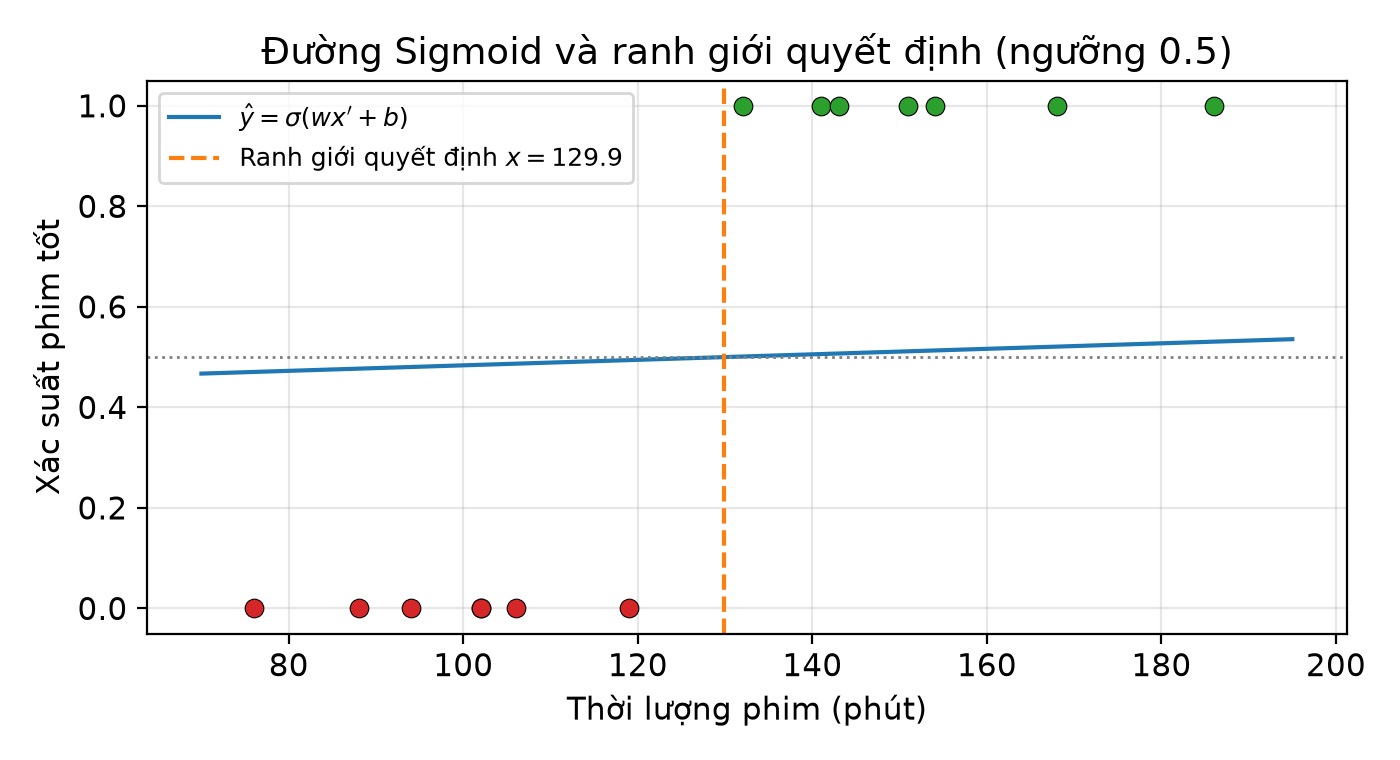
\includegraphics[width=0.82\textwidth]{b2_sigmoid.png}
\end{center}

\subsection*{i) Đồ thị tính toán (Forward Pass và Backward Pass)}

\begin{center}
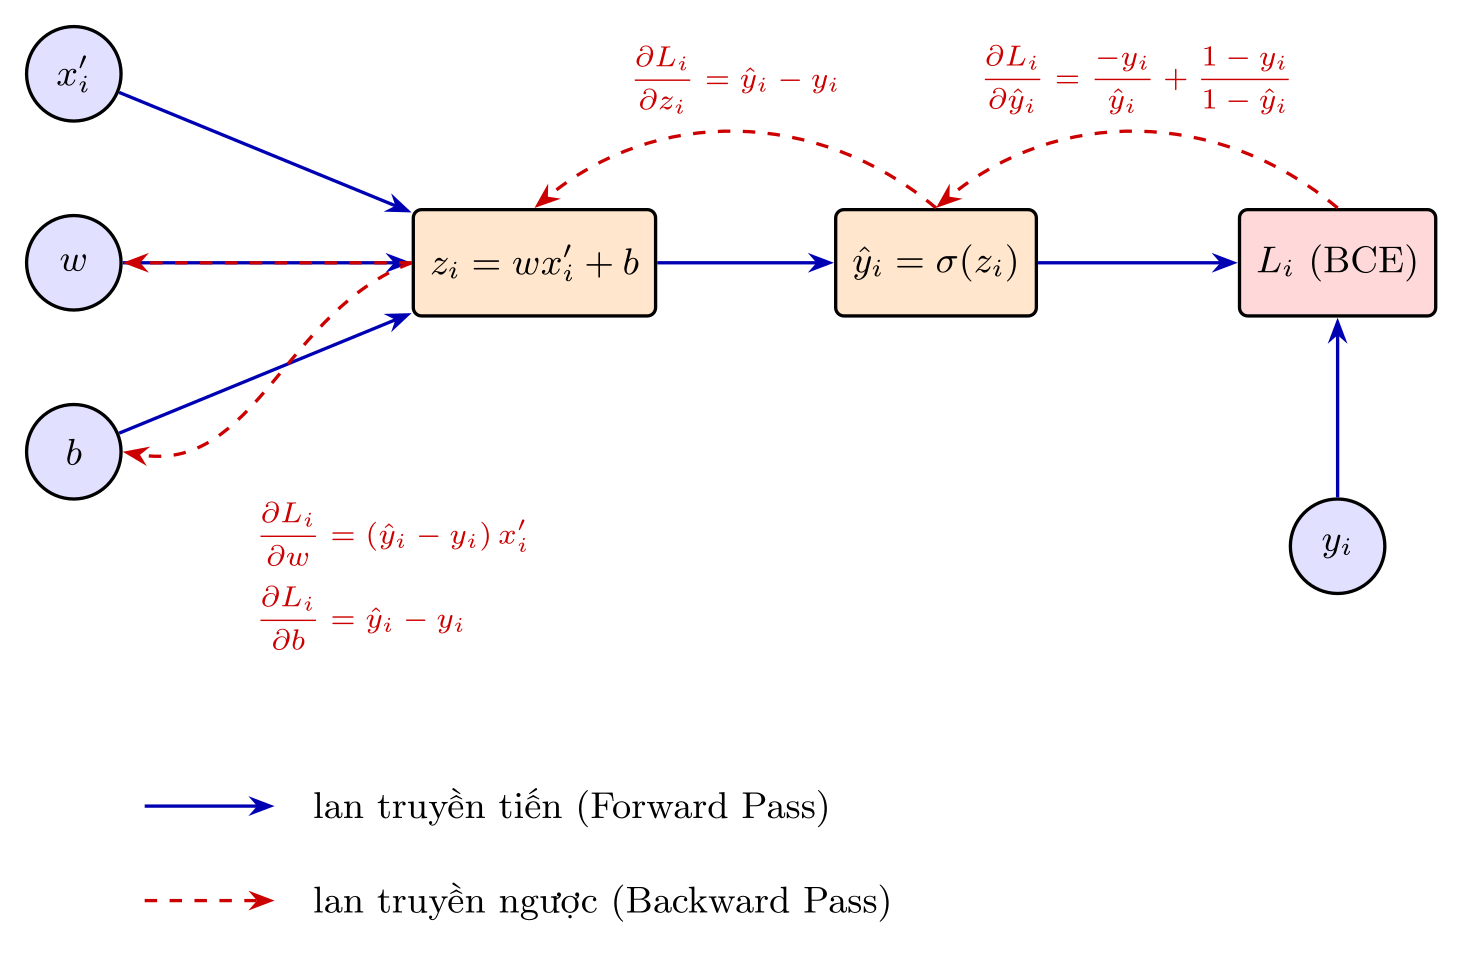
\includegraphics[width=0.98\textwidth]{b2_graph.png}
\end{center}

\subsection*{j) Chương trình PyTorch huấn luyện 1000 lần lặp}

\begin{verbatim}
import numpy as np
import torch

x = torch.tensor([0.04, 0.22, -0.84, 0.48, 0.42, -0.56, -0.22, -0.48,
                  -0.56, 0.26, -1.08, 0.76, -0.72, 1.12], dtype=torch.float32)
y = torch.tensor([1, 1, 0, 1, 1, 0, 0, 0, 0, 1, 0, 1, 0, 1], dtype=torch.float32)

w = torch.zeros(1, requires_grad=True)
b = torch.zeros(1, requires_grad=True)
lr = 0.2
losses = []

for epoch in range(1000):
    y_hat = torch.sigmoid(w * x + b)
    loss = -(y * torch.log(y_hat) + (1 - y) * torch.log(1 - y_hat)).mean()
    losses.append(loss.item())
    loss.backward()
    with torch.no_grad():
        w -= lr * w.grad
        b -= lr * b.grad
    w.grad.zero_()
    b.grad.zero_()

print(w.item(), b.item(), losses[-1])
\end{verbatim}

Kết quả chạy:

\begin{verbatim}
w = 7.6703, b = 0.7685
loss epoch 1    = 0.693147
loss epoch 2    = 0.677941
loss epoch 3    = 0.663341
loss epoch 1000 = 0.066288
\end{verbatim}

\begin{center}
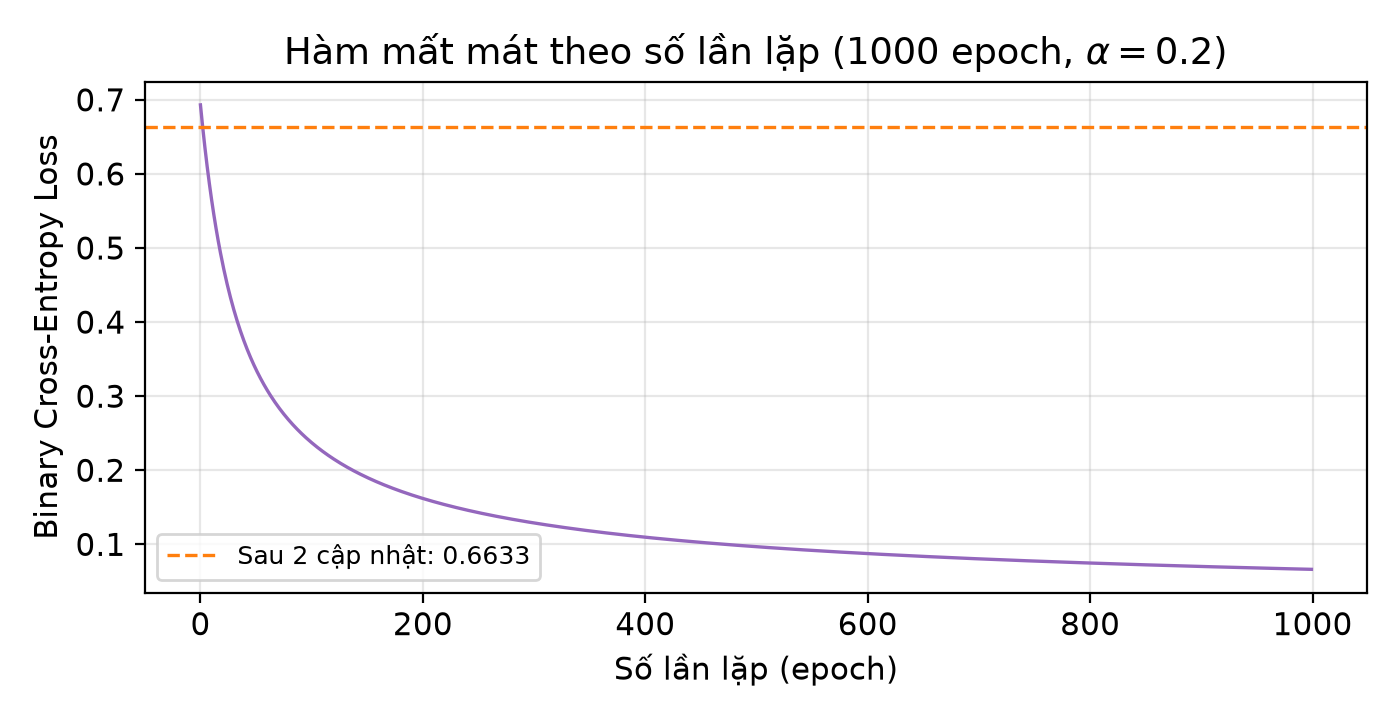
\includegraphics[width=0.82\textwidth]{b2_loss.png}
\end{center}

\textbf{So sánh với kết quả câu (e):} ba giá trị loss đầu tiên của chương trình
(0.693147; 0.677941; 0.663341) trùng khớp hoàn toàn với tính tay tại thời điểm khởi tạo
và sau hai lần cập nhật, xác nhận công thức gradient đã chứng minh là đúng. Sau 1000 lần
lặp, loss giảm còn 0.066288 (so với 0.663341 sau hai lần cập nhật) và mô hình hội tụ về
$w = 7.6703$, $b = 0.7685$ — tức việc chỉ chạy 2 vòng lặp là chưa đủ để hội tụ.

\newpage
\section*{BÀI TẬP 3. ĐỒ THỊ TÍNH TOÁN VÀ LAN TRUYỀN NGƯỢC}

Cho hàm số bốn biến: $J = 3a + 2(4b + 5cd)$ với $a = 2$, $b = 3$, $c = 4$, $d = 5$.
Yêu cầu dùng đồ thị tính toán và quy tắc đạo hàm hàm hợp để tính giá trị hàm số và
đạo hàm riêng theo từng biến.

\subsection*{a) Phân rã biểu thức thành các phép toán cơ bản}

\[ u_1 = 3a, \quad u_2 = 4b, \quad u_3 = cd, \quad u_4 = 5u_3,
   \quad u_5 = u_2 + u_4, \quad u_6 = 2u_5, \quad J = u_1 + u_6. \]

\subsection*{b) Đồ thị tính toán}

\begin{center}
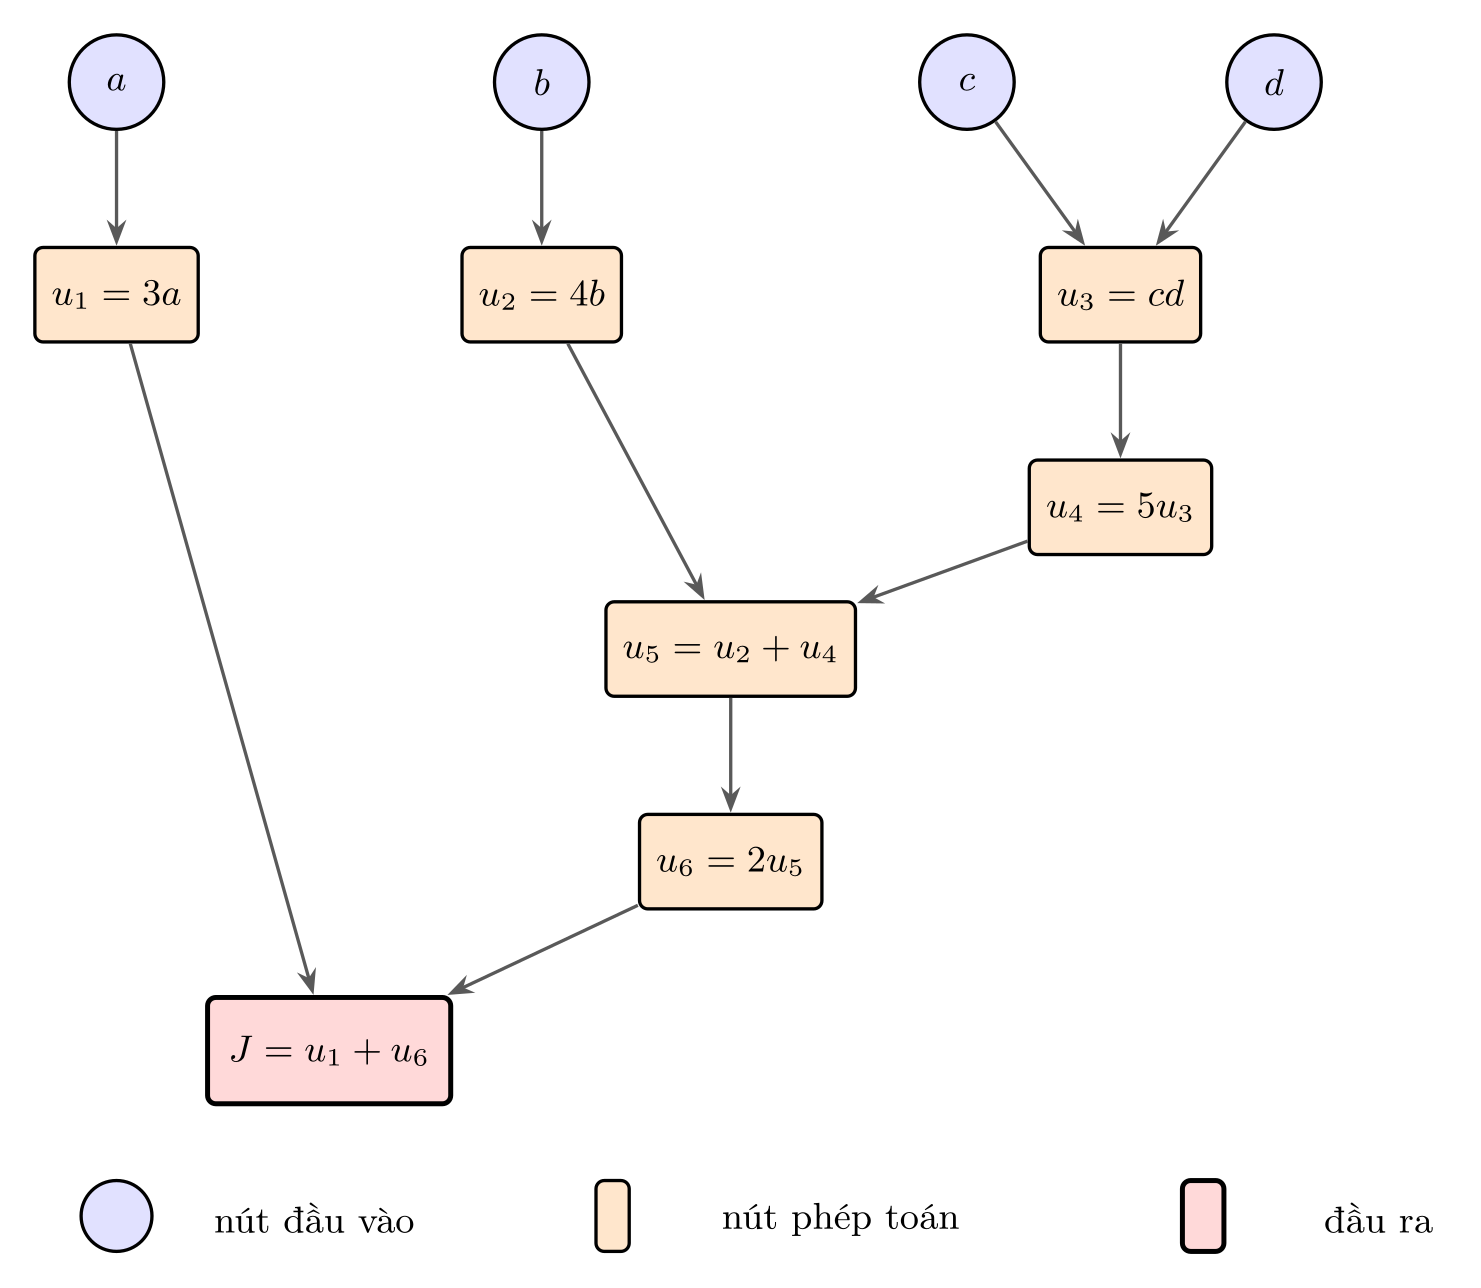
\includegraphics[width=0.95\textwidth]{b3_graph.png}
\end{center}

\subsection*{c) Lan truyền tiến (Forward Pass)}

Tính lần lượt theo thứ tự của đồ thị:

\begin{center}
\begin{tabular}{|c|l|c|}
\hline
Nút & Biểu thức & Giá trị \\
\hline
$u_1$ & $3a = 3\cdot 2$ & 6 \\
$u_2$ & $4b = 4\cdot 3$ & 12 \\
$u_3$ & $cd = 4\cdot 5$ & 20 \\
$u_4$ & $5u_3 = 5\cdot 20$ & 100 \\
$u_5$ & $u_2 + u_4 = 12 + 100$ & 112 \\
$u_6$ & $2u_5 = 2\cdot 112$ & 224 \\
$J$ & $u_1 + u_6 = 6 + 224$ & \textbf{230} \\
\hline
\end{tabular}
\end{center}

\subsection*{d) Đạo hàm cục bộ tại từng nút}

\textbf{Phép cộng} ($u_5 = u_2 + u_4$ và $J = u_1 + u_6$): đạo hàm theo mỗi đầu vào bằng 1.
\[ \frac{\partial u_5}{\partial u_2} = 1, \quad \frac{\partial u_5}{\partial u_4} = 1, \qquad
   \frac{\partial J}{\partial u_1} = 1, \quad \frac{\partial J}{\partial u_6} = 1. \]

\textbf{Phép nhân} (hệ số hằng và tích hai biến):
\[ \frac{\partial u_1}{\partial a} = 3, \qquad \frac{\partial u_2}{\partial b} = 4, \qquad
   \frac{\partial u_4}{\partial u_3} = 5, \qquad \frac{\partial u_6}{\partial u_5} = 2, \]
\[ \frac{\partial u_3}{\partial c} = d = 5, \qquad \frac{\partial u_3}{\partial d} = c = 4. \]

\subsection*{e) Lan truyền ngược (Backward Pass)}

Xuất phát từ $\dfrac{\partial J}{\partial J} = 1$, áp dụng quy tắc dây chuyền:

\begin{center}
\begin{tabular}{|c|l|c|}
\hline
Đại lượng & Cách tính & Giá trị \\
\hline
$\partial J/\partial u_1$ & $1$ & 1 \\
$\partial J/\partial u_6$ & $1$ & 1 \\
$\partial J/\partial u_5$ & $\dfrac{\partial J}{\partial u_6}\cdot 2$ & 2 \\
$\partial J/\partial u_2$ & $\dfrac{\partial J}{\partial u_5}\cdot 1$ & 2 \\
$\partial J/\partial u_4$ & $\dfrac{\partial J}{\partial u_5}\cdot 1$ & 2 \\
$\partial J/\partial u_3$ & $\dfrac{\partial J}{\partial u_4}\cdot 5$ & 10 \\
$\partial J/\partial a$ & $\dfrac{\partial J}{\partial u_1}\cdot 3$ & \textbf{3} \\
$\partial J/\partial b$ & $\dfrac{\partial J}{\partial u_2}\cdot 4$ & \textbf{8} \\
$\partial J/\partial c$ & $\dfrac{\partial J}{\partial u_3}\cdot d$ & \textbf{50} \\
$\partial J/\partial d$ & $\dfrac{\partial J}{\partial u_3}\cdot c$ & \textbf{40} \\
\hline
\end{tabular}
\end{center}

\subsection*{f) Kiểm chứng bằng khai triển trực tiếp}

Khai triển $J$:
\[ J = 3a + 2(4b + 5cd) = 3a + 8b + 10cd. \]
Lấy đạo hàm riêng trực tiếp:
\[ \frac{\partial J}{\partial a} = 3, \qquad \frac{\partial J}{\partial b} = 8, \qquad
   \frac{\partial J}{\partial c} = 10d = 10\cdot 5 = 50, \qquad
   \frac{\partial J}{\partial d} = 10c = 10\cdot 4 = 40. \]
Kết quả trùng khớp hoàn toàn với lan truyền ngược ở câu (e).

\subsection*{g) Một bước Gradient Descent}

Với $\alpha = 0.01$, cập nhật đồng thời:
\[ a' = 2 - 0.01\cdot 3 = 1.97, \qquad b' = 3 - 0.01\cdot 8 = 2.92, \]
\[ c' = 4 - 0.01\cdot 50 = 3.50, \qquad d' = 5 - 0.01\cdot 40 = 4.60. \]

Giá trị hàm mục tiêu sau cập nhật:
\[ J' = 3\cdot 1.97 + 2\bigl(4\cdot 2.92 + 5\cdot 3.50\cdot 4.60\bigr)
      = 5.91 + 2\,(11.68 + 80.5) = 190.27. \]

\textbf{Nhận xét:} hàm mục tiêu giảm từ $230$ xuống $190.27$ (giảm $39.73$), xác nhận bước
cập nhật đi đúng hướng giảm (ngược chiều gradient).

\subsection*{h) Chương trình PyTorch Autograd}

\begin{verbatim}
import torch

a = torch.tensor(2.0, requires_grad=True)
b = torch.tensor(3.0, requires_grad=True)
c = torch.tensor(4.0, requires_grad=True)
d = torch.tensor(5.0, requires_grad=True)

J = 3 * a + 2 * (4 * b + 5 * c * d)
J.backward()

print(J.item())
print(a.grad.item(), b.grad.item(), c.grad.item(), d.grad.item())
\end{verbatim}

Kết quả chạy:

\begin{verbatim}
230.0
3.0 8.0 50.0 40.0
\end{verbatim}

\textbf{So sánh:} PyTorch Autograd cho $J = 230$ và các gradient
$\partial J/\partial a = 3$, $\partial J/\partial b = 8$, $\partial J/\partial c = 50$,
$\partial J/\partial d = 40$ — trùng khớp tuyệt đối với kết quả tính tay bằng
lan truyền ngược ở câu (e) và khai triển trực tiếp ở câu (f).

\begin{center}
---o0o--- \\[0.3cm]
(Hết)
\end{center}

\end{document}
